\documentclass[conference,a4paper,twocolumn]{IEEEtran}
\usepackage{graphicx}
\graphicspath{{images/}}
\DeclareGraphicsExtensions{.png,.jpg,.pdf}
\usepackage{ifpdf}
\usepackage{cite}
\usepackage{todonotes}
\ifCLASSINFOpdf
  % \usepackage[pdftex]{graphicx}
  % declare the path(s) where your graphic files are
  % \graphicspath{{../pdf/}{../jpeg/}}
  % and their extensions so you won't have to specify these with
  % every instance of \includegraphics
  % \DeclareGraphicsExtensions{.pdf,.jpeg,.png}
\else
  % or other class option (dvipsone, dvipdf, if not using dvips). graphicx
  % will default to the driver specified in the system graphics.cfg if no
  % driver is specified.
  % \usepackage[dvips]{graphicx}
  % declare the path(s) where your graphic files are
  % \graphicspath{{../eps/}}
  % and their extensions so you won't have to specify these with
  % every instance of \includegraphics
  % \DeclareGraphicsExtensions{.eps}
\fi

\usepackage[cmex10]{amsmath}
\interdisplaylinepenalty=2500

\usepackage{algorithmic}
\usepackage{array}
\usepackage{mdwmath}
\usepackage{mdwtab}
\usepackage{eqparbox}
\usepackage[tight,footnotesize]{subfigure}
\usepackage[caption=false]{caption}
%\usepackage[font=footnotesize]{subfig}
\usepackage{fixltx2e}
\usepackage{color}
\usepackage{mathtools}


%\usepackage{stfloats}
% stfloats.sty was written by Sigitas Tolusis. This package gives LaTeX2e
% the ability to do double column floats at the bottom of the page as well
% as the top. (e.g., "\begin{figure*}[!b]" is not normally possible in
% LaTeX2e). It also provides a command:
%\fnbelowfloat
% to enable the placement of footnotes below bottom floats (the standard
% LaTeX2e kernel puts them above bottom floats). This is an invasive package
% which rewrites many portions of the LaTeX2e float routines. It may not work
% with other packages that modify the LaTeX2e float routines. The latest
% version and documentation can be obtained at:
% http://www.ctan.org/tex-archive/macros/latex/contrib/sttools/
% Documentation is contained in the stfloats.sty comments as well as in the
% presfull.pdf file. Do not use the stfloats baselinefloat ability as IEEE
% does not allow \baselineskip to stretch. Authors submitting work to the
% IEEE should note that IEEE rarely uses double column equations and
% that authors should try to avoid such use. Do not be tempted to use the
% cuted.sty or midfloat.sty packages (also by Sigitas Tolusis) as IEEE does
% not format its papers in such ways.

% *** PDF, URL AND HYPERLINK PACKAGES ***
%
%\usepackage{url}
% url.sty was written by Donald Arseneau. It provides better support for
% handling and breaking URLs. url.sty is already installed on most LaTeX
% systems. The latest version can be obtained at:
% http://www.ctan.org/tex-archive/macros/latex/contrib/misc/
% Read the url.sty source comments for usage information. Basically,
% \url{my_url_here}.

% *** Do not adjust lengths that control margins, column widths, etc. ***
% *** Do not use packages that alter fonts (such as pslatex).         ***
% There should be no need to do such things with IEEEtran.cls V1.6 and later.
% (Unless specifically asked to do so by the journal or conference you plan
% to submit to, of course. )


% correct bad hyphenation here
\hyphenation{op-tical net-works semi-conduc-tor}


\begin{document}
\title{Elimination of the DC Bus Sixth Harmonic Component in Integrated Modular Motor Drives Using Third Harmonic Injection Method}
\author{\IEEEauthorblockN{Mesut Uğur}
\IEEEauthorblockA{Department of Electrical and Electronics Engineering\\
Middle East Technical University\\
Ankara, Turkey\\
Email: ugurm@metu.edu.tr}
\and
\IEEEauthorblockN{Ozan Keysan}
\IEEEauthorblockA{Department of Electrical and Electronics Engineering\\
Middle East Technical University\\
Ankara, Turkey\\
Email: keysan@metu.edu.tr}
}
\maketitle
\begin{abstract}
%\boldmath
In this paper, a novel method is proposed to enhance the power density of integrated modular motor drive systems by reducing passive element sizes. A method is developed to eliminate the harmonic component on the DC bus which is six times the grid frequency. This harmonic component is present due to natural commutation of the passive diode bridge rectifier in motor drive applications. In conventional drives, bulky LC filters are utilized to reduce the effect of this harmonic component to the motor drive inverter. With this method, DC bus capacitance requirement can be minimized which will enhance the power density and decrease the cost of the overall system. Third harmonic injection is used with modular inverters in an integrated modular motor drive application. Both rectifier and inverter side analytical models are presented, the elimination of the sixth harmonic component is described analytically, and verified by simulations performed on MATLAB/Simulink. A size reduction of \%XXX and a cost reduction of \%YYY is achieved on the DC bus capacitor. The possible adverse effects of third harmonic injection method are also discussed.
\todo[inline]{Abstract'taki sayılar güncellenecek.}
\end{abstract}
\IEEEpeerreviewmaketitle

\section{Introduction}

Introduction will be here.

\vspace{50 mm}

\todo[inline]{Introduction tumuyle eksik}

%\begin{figure}[!t]
%\centering
%\includegraphics[width=8cm]{images/conv_motor_drive}
%\caption{A conventional motor drive block diagram}
%\label{fig:conv_motor_drive}
%\end{figure}


%\begin{figure*}[!t]
%\centerline{\subfloat[Case I]\includegraphics[width=2.5in]{subfigcase1}%
%\label{fig_first_case}}
%\hfil
%\subfloat[Case II]{\includegraphics[width=2.5in]{subfigcase2}%
%\label{fig_second_case}}}
%\caption{Simulation results}
%\label{fig_sim}
%\end{figure*}


% The following is an example of commenting a large section
\iffalse
\begin{table}[htp]
\renewcommand{\arraystretch}{1.3}
\caption{An Example of a Table}
\label{table_example}
\centering
\begin{tabular}{|c|c|c|}
\hline
One & Two & a\\
\hline
Three & Four & a\\
\hline
Three & Four & b\\
\hline
\end{tabular}
\end{table}
\fi

Most studies consider only one side for DC link characterisation or filter component optimization, although they should be considered simultaneously. This research aims at modeling the system as a whole, investigating the effect of harmonic components injected to the DC link from both sides and eliminating the low frequency harmonic due to the rectifier side by using the modular structure of the inverter side.

\section{Problem definition}
%analytical Rectifier model, 6th harmonic component %injection, LC filter characteristics

A conventional motor drive system block diagram is shown in Fig. \ref{fig:conv_motor_drive}. The rectifier and inverter are connected via the DC link, therefore a harmonic component injected from one side may be reflected to the other side, disrupting its operation. For systems having two active converters on both sides such as back-to-back converters, the only fluctuations seen on the DC link voltage are high frequency components which are directly related to the switching frequencies of each side. On the other hand, in case of passive converters such as diode bridge rectifiers, low frequency components emerge on the DC link voltage which are related to the grid supply frequency. Since grid frequency is usually much smaller than the switching frequencies applied to active converters, filtering of fluctuations on the DC link requires much larger and more expensive filter components in case of passive rectifiers.
\begin{figure}[h]
  \centering
  \includegraphics[width=9cm]{conv_motor_drive}
  \caption{A conventional motor drive system block diagram}
  \label{fig:conv_motor_drive}
\end{figure}

The diode bridge rectifier is a natural-commutated converter, circuit schematic of which is shown in Fig. \ref{fig:rect_circuit}. A second order LC filter which is of low-pass type is usually utilized at the rectifier output for filtering. In this section, the harmonic content of the rectifier output voltage and the effect of filtering are shown analytically.

\begin{figure}[h]
  \centering
  \includegraphics[width=9cm]{rect_circuit}
  \caption{Diode bridge rectifier circuit diagram}
  \label{fig:rect_circuit}
\end{figure}

The supply voltages are shown in \ref{ahmet}-\ref{mehmet}, where $V_m$ is the RMS value of the supply voltage and $f_s$ is the supply frequency. With this configuration, integer multiples of the harmonic component frequency of which is six times the grid frequency $f_s$ are present on the rectifier output voltage in addition to the DC component as shown in \ref{hasan}. 

\begin{equation} \label{ahmet}
v_{sa}(t) = \sqrt{2}V_msin(2\pi f_s t)
\end{equation}
\begin{equation} \label{eq:2}
v_{sb}(t) = \sqrt{2}V_msin(2\pi f_s t-2\pi/3)
\end{equation}
\begin{equation} \label{mehmet}
v_{sc}(t) = \sqrt{2}V_msin(2\pi f_s t-4\pi/3)
\end{equation}
\begin{equation} \label{hasan}
v_{dc}(t) = \frac{3\sqrt{3}}{\pi} \bigg[1-\sum_{k=1}^{\infty} \frac{2}{36k^2-1}cos(6k\omega_{0}t)\bigg] 
%\sqrt{2}V_msin(2\pi f_s t)
\end{equation}

The transfer function between $v_{load}$ and $v_{dc}$ is obtained to show the characteristics of the filter as in \ref{eq:tf}. Magnitude and phase of the harmonic components that are of interest are obtained from this model and they are later used in the implementation of the proposed method.

\begin{equation} \label{eq:tf}
H(jw) = \frac{v_{L}(jw)}{v_{dc}(jw)} = \frac{R_{L}}{R_{L}(1-w^2L_{dc}C_{dc})+jwL_{dc}}
\end{equation}

A simulation is performed for the verification of these analytical models on MATLAB/Simulink, for 400V line-to-line grid voltage at 50 Hz, filter inductance of 1 mH, filter capacitance of 4 mF and load resistance of 10 $\Omega$. In Fig. \ref{fig:rect_wave}, the three-phase input voltages, the rectifier output voltage and the filtered load voltage waveforms are shown. In Fig. \ref{fig:fft1} and \ref{fig:fft2}, the harmonic spectra of rectifier output voltage and load voltage are shown, respectively.
\begin{figure}[h]
  \centering
  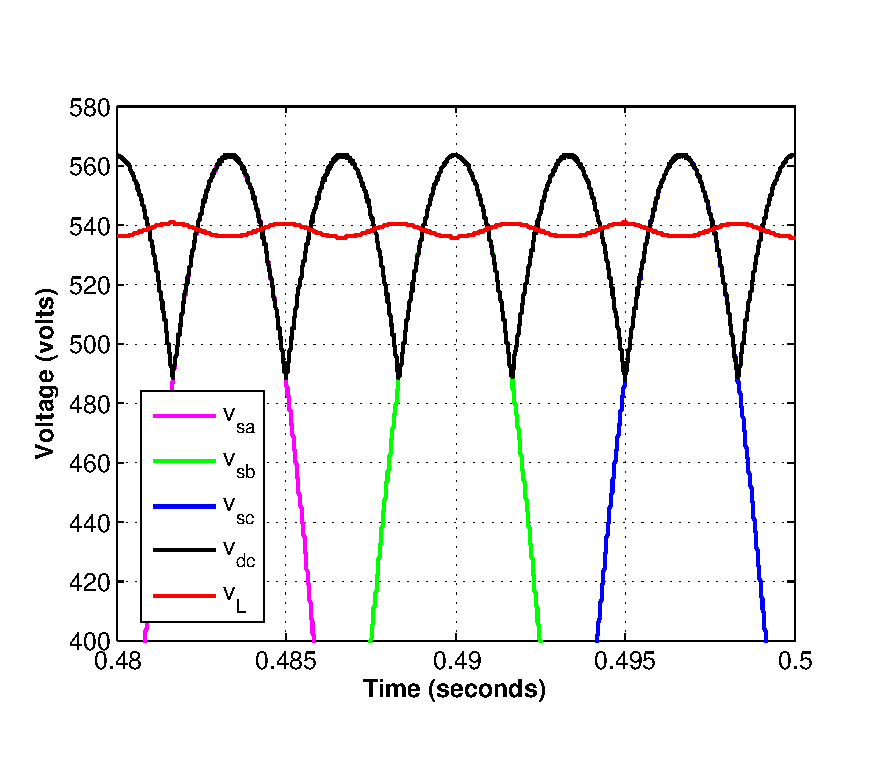
\includegraphics[width=8cm]{images/rect_wave}
  \caption{Diode bridge rectifier input and output waveforms}
  \label{fig:rect_wave}
\end{figure}
A load voltage peak-to-peak ripple of 1\% is usually aimed in case of motor drive inverter applications and the filter values are adjusted here such that a ripple of 0.9\% is obtained. The inductance value is usually determined by the current ripple on this inductor and it has minor effect on the load voltage ripple. Capacitance values on the DC link are usually in a few hundred microfarad range when only high frequency fluctuations are considered, however in this case, capacitance values in milifarad range are needed.


\begin{figure}[htp]
  \centering
  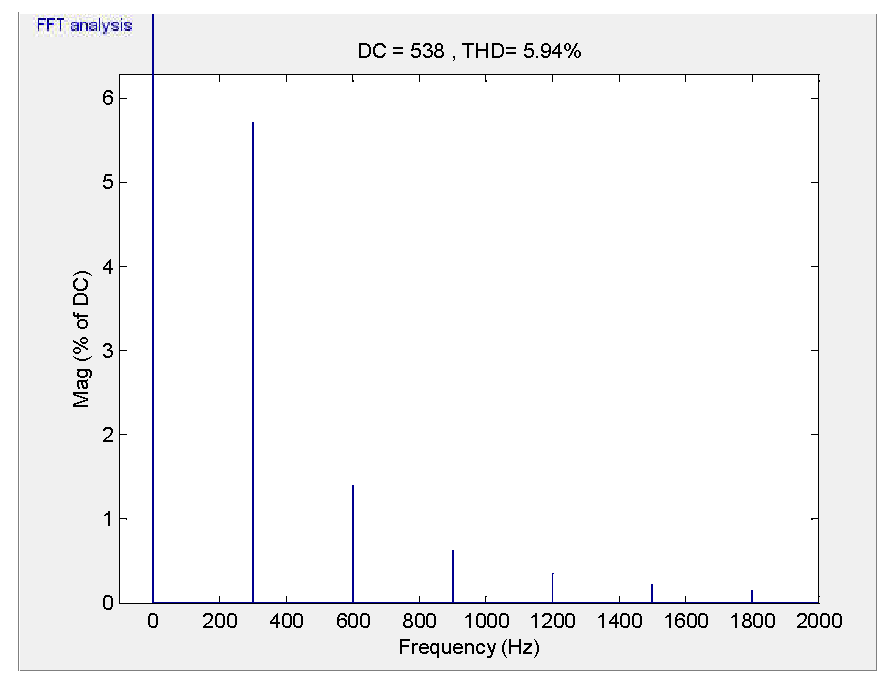
\includegraphics[width=8cm]{images/fft1}
  \caption{Harmonic spectrum of rectifier output voltage}
  \label{fig:fft1}
\end{figure}
\begin{figure}[h]
  \centering
  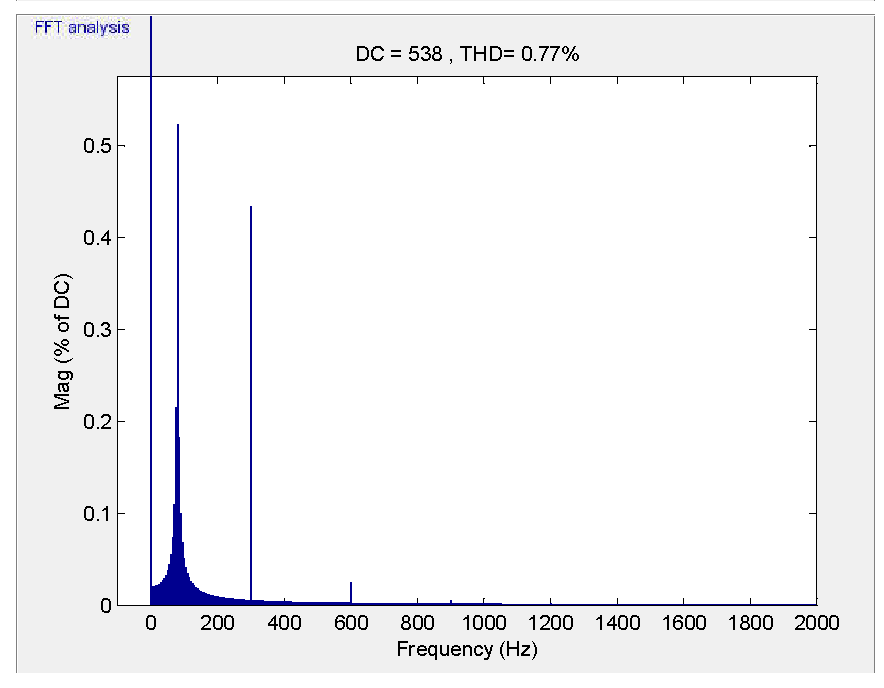
\includegraphics[width=8cm]{images/fft2}
  \caption{Harmonic spectrum of load voltage}
  \label{fig:fft2}
\end{figure}

In IMMD applications, decreasing the volume of the passive elements is a major challenge due to having small volume. Therefore, integration of the motor drive with passive rectifiers to the motor is a problem.

\todo[inline]{buraya \% 30unu kaplıyor gibi istatistikler gelebilir. IMMD ile ilgili olan kisim baglanacak. Harmonic spectrum lar duzenlenecek.}


\section{Description of the proposed method}
In the proposed method, a harmonic component which is six times the grid frequency is aimed to be created at the inverter DC input such that there will be no low order harmonic current flowing through the DC link capacitor, as shown in Fig. \ref{fig:6th}. By doing so, the DC link capacitance requirement can be reduced significantly.
\begin{figure}[htp]
  \centering
  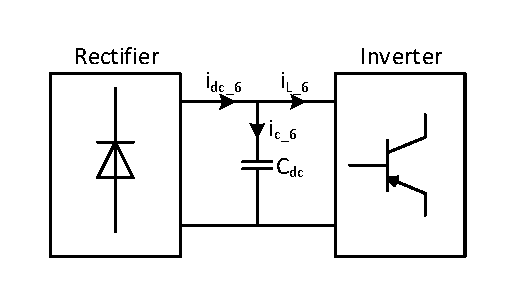
\includegraphics[width=8cm]{images/method}
  \caption{The proposed method}
  \label{fig:6th}
\end{figure}
The harmonic component is created by injecting zero sequence third harmonic components at the motor side. Voltages and current expressions of one inverter module with zero sequence third harmonic injection are shown in \ref{eq:volta}-\ref{eq:currc}.
\begin{equation} \label{eq:volta}
v_a(t) = V_1sin(2\pi ft-\phi_{1v})+V_3sin(6\pi ft-\phi_{3v})
\end{equation}
\begin{equation} \label{voltb}
v_b(t) = V_1sin(2\pi ft-2\pi/3-\phi_{1v})+V_3sin(6\pi ft-\phi_{3v})
\end{equation}
\begin{equation} \label{eq:voltc}
v_c(t) = V_1sin(2\pi ft-4\pi/3-\phi_{1v})+V_3sin(6\pi ft-\phi_{3v})
\end{equation}
\begin{equation} \label{eq:curra}
i_a(t) = I_1sin(2\pi ft-\phi_{1i})+I_3sin(6\pi ft-\phi_{3i})
\end{equation}
\begin{equation} \label{eq:currb}
i_b(t) = I_1sin(2\pi ft-2\pi/3-\phi_{1i})+I_3sin(6\pi ft-\phi_{3i})
\end{equation}
\begin{equation} \label{eq:currc}
i_c(t) = I_1sin(2\pi ft-4\pi/3-\phi_{1i})+I_3sin(6\pi ft-\phi_{3i})
\end{equation}

Let us make the definitions shown in \ref{eq:def1}-\ref{eq:def2}, where v denotes voltage, i denotes current, k denotes fundamental component and l denotes third harmonic component.
\begin{equation} \label{eq:def1}
\phi_{kl-p} = \phi_{kv}+\phi_{li}
\end{equation}
\begin{equation} \label{eq:def2}
\phi_{kl-n} = \phi_{kv}+\phi_{li}
\end{equation}

\iffalse
\begin{equation} \label{eq:9}
\phi_{13p} = \phi_{1v}+\phi_{3i}
\end{equation}
\begin{equation} \label{eq:10}
\phi_{31p} = \phi_{3v}+\phi_{1i}
\end{equation}
\begin{equation} \label{eq:11}
\phi_{11n} = \phi_{1v}-\phi_{1i}
\end{equation}
\begin{equation} \label{eq:12}
\phi_{33n} = \phi_{3v}-\phi_{3i}
\end{equation}
\begin{equation} \label{eq:13}
\phi_{13n} = \phi_{1v}-\phi_{3i}
\end{equation}
\begin{equation} \label{eq:14}
\phi_{31n} = \phi_{3v}-\phi_{1i}
\end{equation}
\fi


The instantaneous power expression for each phase are shown in \ref{eq:pa}-\ref{eq:pc}.

\begin{equation}
\label{eq:pa}
\begin{multlined}
p_a(t) = 
\frac{V_1I_1}{2} \bigg \lbrack cos(\phi_{11n})-cos(4\pi ft-\phi_{11p}) \bigg \rbrack
\\
+
\frac{V_1I_3}{2} \bigg \lbrack cos(4\pi ft+\phi_{13n})-cos(8\pi ft-\phi_{13p}) \bigg \rbrack
\\
+
\frac{V_3I_1}{2} \bigg \lbrack cos(4\pi ft-\phi_{31n})-cos(8\pi ft-\phi_{31p}) \bigg \rbrack
\\
+
\frac{V_3I_3}{2} \bigg \lbrack cos(\phi_{33n})-cos(12\pi ft-\phi_{33p}) \bigg \rbrack,
\end{multlined}
\end{equation}

\begin{equation}
\label{eq:pb}
\begin{multlined}
p_b(t) = 
\frac{V_1I_1}{2} \bigg \lbrack cos(\phi_{11n})-cos(4\pi ft-4\pi/3-\phi_{11p}) \bigg \rbrack
\\
+
\frac{V_1I_3}{2} \bigg \lbrack cos(4\pi ft+ 2\pi/3+\phi_{13n})-cos(8\pi ft-2\pi/3-\phi_{13p}) \bigg \rbrack
\\
+
\frac{V_3I_1}{2} \bigg \lbrack cos(4\pi ft+2\pi/3-\phi_{31n})-cos(8\pi ft-2\pi/3-\phi_{31p}) \bigg \rbrack
\\
+
\frac{V_3I_3}{2} \bigg \lbrack cos(\phi_{33n})-cos(12\pi ft-\phi_{33p}) \bigg \rbrack,
\end{multlined}
\end{equation}

\begin{equation}
\label{eq:pc}
\begin{multlined}
p_c(t) = 
\frac{V_1I_1}{2} \bigg \lbrack cos(\phi_{11n})-cos(4\pi ft-8\pi/3-\phi_{11p}) \bigg \rbrack
\\
+
\frac{V_1I_3}{2} \bigg \lbrack cos(4\pi ft+ 4\pi/3+\phi_{13n})-cos(8\pi ft-4\pi/3-\phi_{13p}) \bigg \rbrack
\\
+
\frac{V_3I_1}{2} \bigg \lbrack cos(4\pi ft+4\pi/3-\phi_{31n})-cos(8\pi ft-4\pi/3-\phi_{31p}) \bigg \rbrack
\\
+
\frac{V_3I_3}{2} \bigg \lbrack cos(\phi_{33n})-cos(12\pi ft-\phi_{33p}) \bigg \rbrack,
\end{multlined}
\end{equation}

The total instantaneous power becomes as in \ref{eq:pt}. As seen, all the frequency components which are two times and four times the fundamental frequency are cancelled, leaving two DC components and a component at six times the fundamental frequency. The last term will be used in this method for the cancellation of the sixth harmonic injected by the rectifier.

\begin{equation}
\label{eq:pt}
\begin{multlined}
p_{total}(t) = 
\frac{V_1I_1}{2} \bigg \lbrack cos(\phi_{11n}) \bigg \rbrack
+
\frac{V_3I_3}{2} \bigg \lbrack cos(\phi_{33n}) \bigg \rbrack
\\
+
\frac{V_3I_3}{2} \bigg \lbrack cos(12\pi ft-\phi_{33p}) \bigg \rbrack
\end{multlined}
\end{equation}




\section{Implementation of the method and practical issues}

This method is proposed for IMMD applications where selection of number of inverter modules, number of stator phases etc. are flexible. This makes the application of the method more convenient for IMMD applications. The schematic diagram of the segmented stator and modular inverters is shown in Fig. \ref{fig:segmented}. The inverters can be connected in series, parallel or both in IMMD configurations. Each technique has its own advantages and drawbacks. In this paper, a machine with 4 pole pairs is considered, each having three phases. All the modules are connected in parallel on the DC bus.
\todo[inline]{Bu konuyu daha iyi aciklayalim mi}

\begin{figure}[htp]
  \centering
  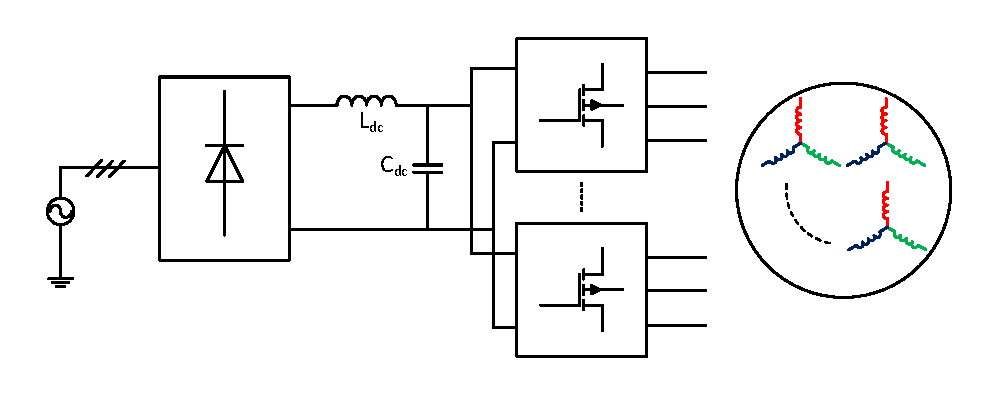
\includegraphics[width=9cm]{segmented}
  \caption{The schematic of the segmented stator and modular inverters}
  \label{fig:segmented}
\end{figure}

It has been shown that, with conventional three-phase connection, injection of third harmonic is impossible, regardless of the winding connection being delta or wye, due to the nature of the three-phase. Therefore, in this paper, an IMMD scheme is proposed such that each stator coil is fed by a separate single-phase bridge inverter.

The conventional connection and the proposed connection are shown in Fig. \ref{fig:conv_conn}, for only one pole pair.

%\begin{figure}[htp]
%  \centering
%  \includegraphics[width=8cm]{images/prop_conn}
%  \caption{Conventional connection and proposed %connection}
%  \label{fig:prop_conn}
%\end{figure}

\begin{figure}[] 
\centering
\subfigure[]{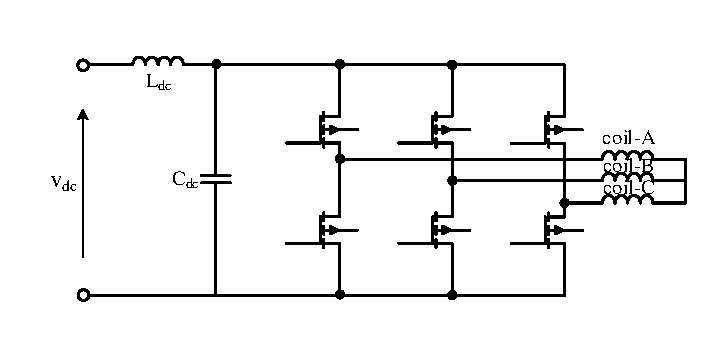
\includegraphics[width=2.5in]{conv_conn}\label{conv_conn}} \hfil 
\subfigure[]{\includegraphics[width=2.5in]{prop_conn}\label{prop_conn}}
\caption{Inverter schematic a) Conventional, b) Proposed.} 
\label{fig:conv_conn} 
\end{figure}

With this connection, each H-bridge module has the voltage to which third harmonic component is added. All the added components have the same phase so that a harmonic component which is six times the grid frequency is obtained as discussed in Section III. Apart from the elimination of the sixth harmonic component and hence reducing the capacitor size and RMS current requirement, this method has some drawbacks which have been discussed as follows: 
\begin{enumerate}
  \item Number of power semiconductor devices, and hence power semiconductor cost is increased. 
  \item Power semiconductor device conduction and switching losses are increased for two reasons. First of all, the same current now flows through two devices at the same time instead of one, for each coil. Secondly, the injected third harmonic current introduces additional conduction losses to the devices.
  \item Motor copper losses and core losses are increased due to the injection of the third harmonic component. The RMS current is increased which is directly related to the copper loss. Additionally, the third harmonic component, which does not contribute to the average useful torque creates eddy current losses on the rotor.
  \item Increase of the power electronics and motor losses makes the cooling of the system more difficult, which has been already difficult due to the integrated structure.
  \item The injection of the third harmonic may yield low frequency torque ripple on the shaft. It has been shown analytically that, if there is no third space harmonic, the injection does not cause any torque ripple. On the other hand, even if a small third space harmonic is present on the motor, it will cause torque ripple.
\end{enumerate}
Furthermore, this method may also bring some additional advantages as follows:
\todo[inline]{Buraya daha detayli girilmesi lazim}

\begin{enumerate}
  \item Separating all the phases apart will further enhance the modularity of the motor drive system.
  \item Increased modularity neler getiriyor?
  \item Torque ripple'a yonelik neler yapilabilir motor tarafinda?
\end{enumerate}

The adverse effects of the method are also studied in addition to the benefits of the method for the reduction of passive element size and cost, and its results are also included in Section V.

\section{Results}
The proposed method is verified by simulations carried out in MATLAB/Simulink and the results of the enhanced performance on the Dc link is obtained. Moreover, the results for the drawbacks are also obtained. Then, benefits of the method are discussed quantitatively and the price that is paid to obtain these benefits are obtained. In Table \ref{table:sim_param}, parameters used in the simulation work are listed.

\begin{table}[h]
\renewcommand{\arraystretch}{1.4}
\caption{Parameters used in the simulation}
\label{table:sim_param}
\centering
\begin{tabular}{|c|c|c|c|}
\hline
Total output power & 10 kW & Switching frequency & 20 kHz\\
\hline
Motor fund. frequency & 50 Hz & Supply frequency & 50 Hz\\
\hline
Supply voltage & 400 V & Motor voltage & 400 V\\
\hline
Three-phase modules & 4 & Parallel connected modules & 4\\
\hline
DC Bus filter inductance & 1 mH & DC bus filter capacitance & 100 uF\\
\hline
Some motor parameters & abc & Some other parameters & xyz\\
\hline
\end{tabular}
\end{table}

The rectifier output current ($i_{dc}$), the inverter input current ($i_{inv}$), and DC link capacitor current ($i_{c}$) are shown in Fig. \ref{fig:main_currents}. \todo[inline]{Elde edilecek}. The DC link capacitor current is shown in Fig. \ref{fig:cap_current} with and without the method, with 0.2 mF capacitance value. \todo[inline]{Elde edilecek}. The same figure is shown in Fig. \ref{fig:cap_current2} with 3 mF capacitance value. \todo[inline]{Elde edilecek}.

\begin{figure}[h]
  \centering
  \includegraphics[width=8cm]{images/sample}
  \caption{The rectifier output current, the inverter input current, and DC link capacitor current}
  \label{fig:main_currents}
\end{figure}

\begin{figure}[h]
  \centering
  \includegraphics[width=8cm]{images/sample}
  \caption{DC link capacitor current with and without the method ($C_{dc} = 0.2 mF$)}
  \label{fig:cap_current}
\end{figure}

\begin{figure}[h]
  \centering
  \includegraphics[width=8cm]{images/sample}
  \caption{DC link capacitor current with and without the method ($C_{dc} = 3 mF$)}
  \label{fig:cap_current2}
\end{figure}

Motor line currents for only one three-phase module are shown in Fig. \ref{fig:motor_current}. \todo[inline]{Elde edilecek}. Transistor voltage and current waveforms for only one H-bridge module are shown in Fig. \ref{fig:transistor_current}. \todo[inline]{Elde edilecek, The increase on the conduction losses of the switches and the copper losses of the windings}.
 
In Fig. \ref{fig:inverter_current}, inverter currents are shown along with the DC link current, showing the creation of the sixth harmonic component. \todo[inline]{Elde edilecek}.

\begin{figure}[h]
  \centering
  \includegraphics[width=8cm]{images/sample}
  \caption{The motor line currents for only one three-phase module}
  \label{fig:motor_current}
\end{figure}

\begin{figure}[h]
  \centering
  \includegraphics[width=8cm]{images/sample}
  \caption{Transistor voltage and current waveforms for only one H-bridge module}
  \label{fig:transistor_current}
\end{figure}

\begin{figure}[h]
  \centering
  \includegraphics[width=8cm]{images/sample}
  \caption{Inverter currents are shown along with the DC link current}
  \label{fig:inverter_current}
\end{figure}

The requirement for the DC bus capacitor is reduced in two aspects: capacitance and RMS current requirement. The capacitance requirement is reduced since the DC link voltage ripple is now reduced. Moreover, since the low order harmonic components now do not flow through the capacitor, the RMS current requirement is also reduced.

The same performance is obtained by using a capacitance which is 20 times smaller.

The sixth harmonic current decreased to its 5 percent.

The overall RMS current decreased to its 50 percent.

When comparing the two cases, two capacitor banks, which are commercially available off-the-shelf products, are selected with the requirements and they are compared in terms of:
- Cost
- Power density
- Lifetime
- Operating Temperature
- Loss

In all these aspects, xyz percent better or worse, burda tablo mu versek...

DC bus capacitance requirement is directly related to the percent peak-to-peak voltage ripple constraint on the DC bus voltage. Therefore, application of the proposed method has no significant effect on the capacitance, however the RMS current requirement decreases significantly.
Film capacitors has high RMS current ratings, but their capacitance per volume is low. On the contrary, aluminium electrolytic capacitors have low RMS current rating, but very high capacitance ratings per volume. Therefore, the proposed method will not have much effect when film capacitors are used, unless the switching frequency is higher than 150 kHz. On the other hand, overall cost and volume can be reduced significantly if aluminium electrolytic capacitors are used.
This will have the effects of:
- Lower cost
- Higher power density
- Lifetime may be extended

In this paper, a case is considered where the grid supply frequency and the motor fundamental frequency are close to each other, which may be the case most of the time, in some applications. On the other hand, in some other applications a variety of frequencies may be needed. When the difference is high, the adverse effects will be more dominant. One precaution to deal with this is using the modularity of the system such that the number of poles to be used can be changed electronically, without needing any additional connections or some mechanical intervention. By doing so, speed range can be enhanced with a smaller range of frequencies and this method can be made more feasible even for applications that need a wide speed range.


\section{Conclusion}
The conclusion goes here.


\section*{Acknowledgment}

The authors would like to thank...



\begin{thebibliography}{1}

\bibitem{IEEEhowto:kopka}
H.~Kopka and P.~W. Daly, \emph{A Guide to \LaTeX}, 3rd~ed.\hskip 1em plus
  0.5em minus 0.4em\relax Harlow, England: Addison-Wesley, 1999.

\end{thebibliography}


\end{document}